The MusEEG package is a Python package containing useful classes that aid developers in preprocessing and classifying EEG data, creating MIDI objects, instantiating an OSC client, and designing a Brain-Computer Music Interface that allows a user to trigger MIDI events and OSC messages from performing facial expressions. The MusEEG project is available as an open-source package and can be downloaded from its GitHub repository\footnote{To access the MusEEG GitHub repository visit: https://github.com/hugofloresgarcia/MusEEG}.

\section{Regarding Open Source Privacy Concerns}
Due to the open-source, train-it yourself nature of the MusEEG project, a particular subject’s EEG data is handled by only the subject himself, as it is advised that the neural network model is trained for a single individual only for higher classification accuracy. 
In order for a user to create their own personalized neural network model, the user must first download the MusEEG package from GitHub to their personal computer. The MusEEG eegData module’s training methods facilitate the data collection process, organizing and labeling the training data into processing chunks inside the MusEEG directory. The processed and labeled training data is then used to create and train a new neural network model customized to the user’s training data, which will also be stored inside the MusEEG directory. 
It should be noted that all of the EEG data acquired by the user is processed and saved inside the user’s local MusEEG directory and is never uploaded to the web. Thus, each user’s EEG data and trained neural network models reside inside the same user’s computer, and are never shared, accessed, or viewed by any other subject without the original user’s consent and deliberate intent.


\section{Demo Application}
  \begin{figure}[htbp!]
	\centering
		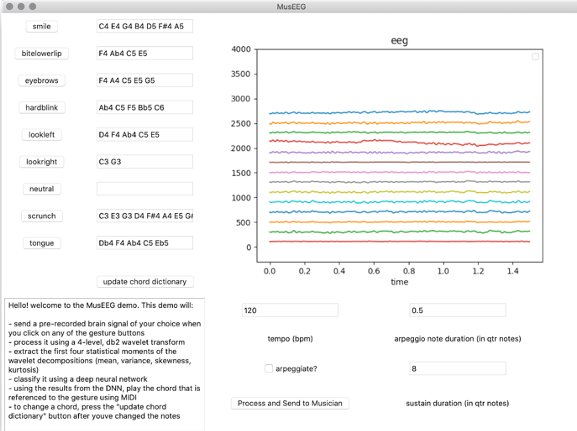
\includegraphics[width=1\columnwidth]{demoApp.png}
	\caption{Demo Application GUI}
	\label{fig:demoApp}
\end{figure} 

The demo application was created as a static proof-of-concept that provides a demonstration of the basic functionality of the MusEEG package. In short, the MusEEG demo application lets the user perform the following actions:
\begin{itemize}
  \item	Create a MIDI chord dictionary by entering note names next to the desired facial expression.
\item	Load a pre-recorded facial expression sample from the dataset.
\item	Process the pre-recorded sample using wavelet decomposition as well as perform the statistical moments calculation.
\item	Classify the pre-recorded facial expression sample using the \textit{bigBrain} classifier.
\item	Refer the resulting facial expression from the classification result to its corresponding chord in the MIDI dictionary.
\item	Send the MIDI event to a virtual MIDI port with a set of music-related control parameters (arpeggiation, tempo, sustain duration, arpeggio note duration). 
\end{itemize}


\subsection{The Facial Expression Buttons and Chord Dictionary}
The top left corner of the demo application allows the user to load a random sample from the existing facial expression dataset by pressing on one of the facial expression buttons. Once loaded, the 14-channel raw EEG signal will be plotted in the plot box.
Next to each facial expression button is a text entry field that allows the user to define the set of notes that will be played when the facial expression is sent to the main processor. Note: whenever the user changes notes in the chord dictionary, the update chord dictionary button must be pressed in order for the changes to take effect.

\subsection{Process and Send Button}
The process and send button performs the following actions:\\
1.	wavelet transform of raw EEG signal\\
2.	statistical moment calculations of wavelet decomposition vectors\\
3.	creates ANN input array from extracted stat moments\\
4.	the ANN classifies the signal into either of the available facial expressions\\
5.	the facial expression is referred to its matching chord in the chord dictionary, and a chord object is created from the matching chord\\
6.	the playchord method is called on the chord object, sending a MIDI message according to the additional control parameters\

\subsection{Additional Controls}
Additional controls are available for the demo app:\\
•	arpeggiate: if the box is checked, the chord will play in an arpeggio as opposed to vertically.\\
•	sustain duration: indicates how long (in quarter notes) the chord will be sustained (only applied if arpeggiate is unchecked)\\
•	arpeggio note duration: indicates how long (in quarter notes) each note in the arpeggio will last.\\

\pagebreak
\section{Real-Time Processing}
%A real-time application of the brain-computer interface is currently in progress. The current iteration of the real-time application consists of a multithreaded process (Figure~\ref{fig:realTimeFlowChart}). This method has not yet been tested properly and may need adjustments in order to ensure proper performance.

Two different real-time processing algorithms were designed for MusEEG. Though both use the same preprocessing and classification methods (discussed in \autoref{chap:dataAcquisition}), their methods for segmenting the raw EEG data into analyzable chunks are distinct. 

\subsection{Real Time Processing with \textit{smallBrain} Wake Up}
A flowchart describing the real-time processing workflow using \textit{smallBrain} wake up is described in (Figure~\ref{fig:realTimeFlowChart}).
 
 \begin{figure}[H]
	\centering
		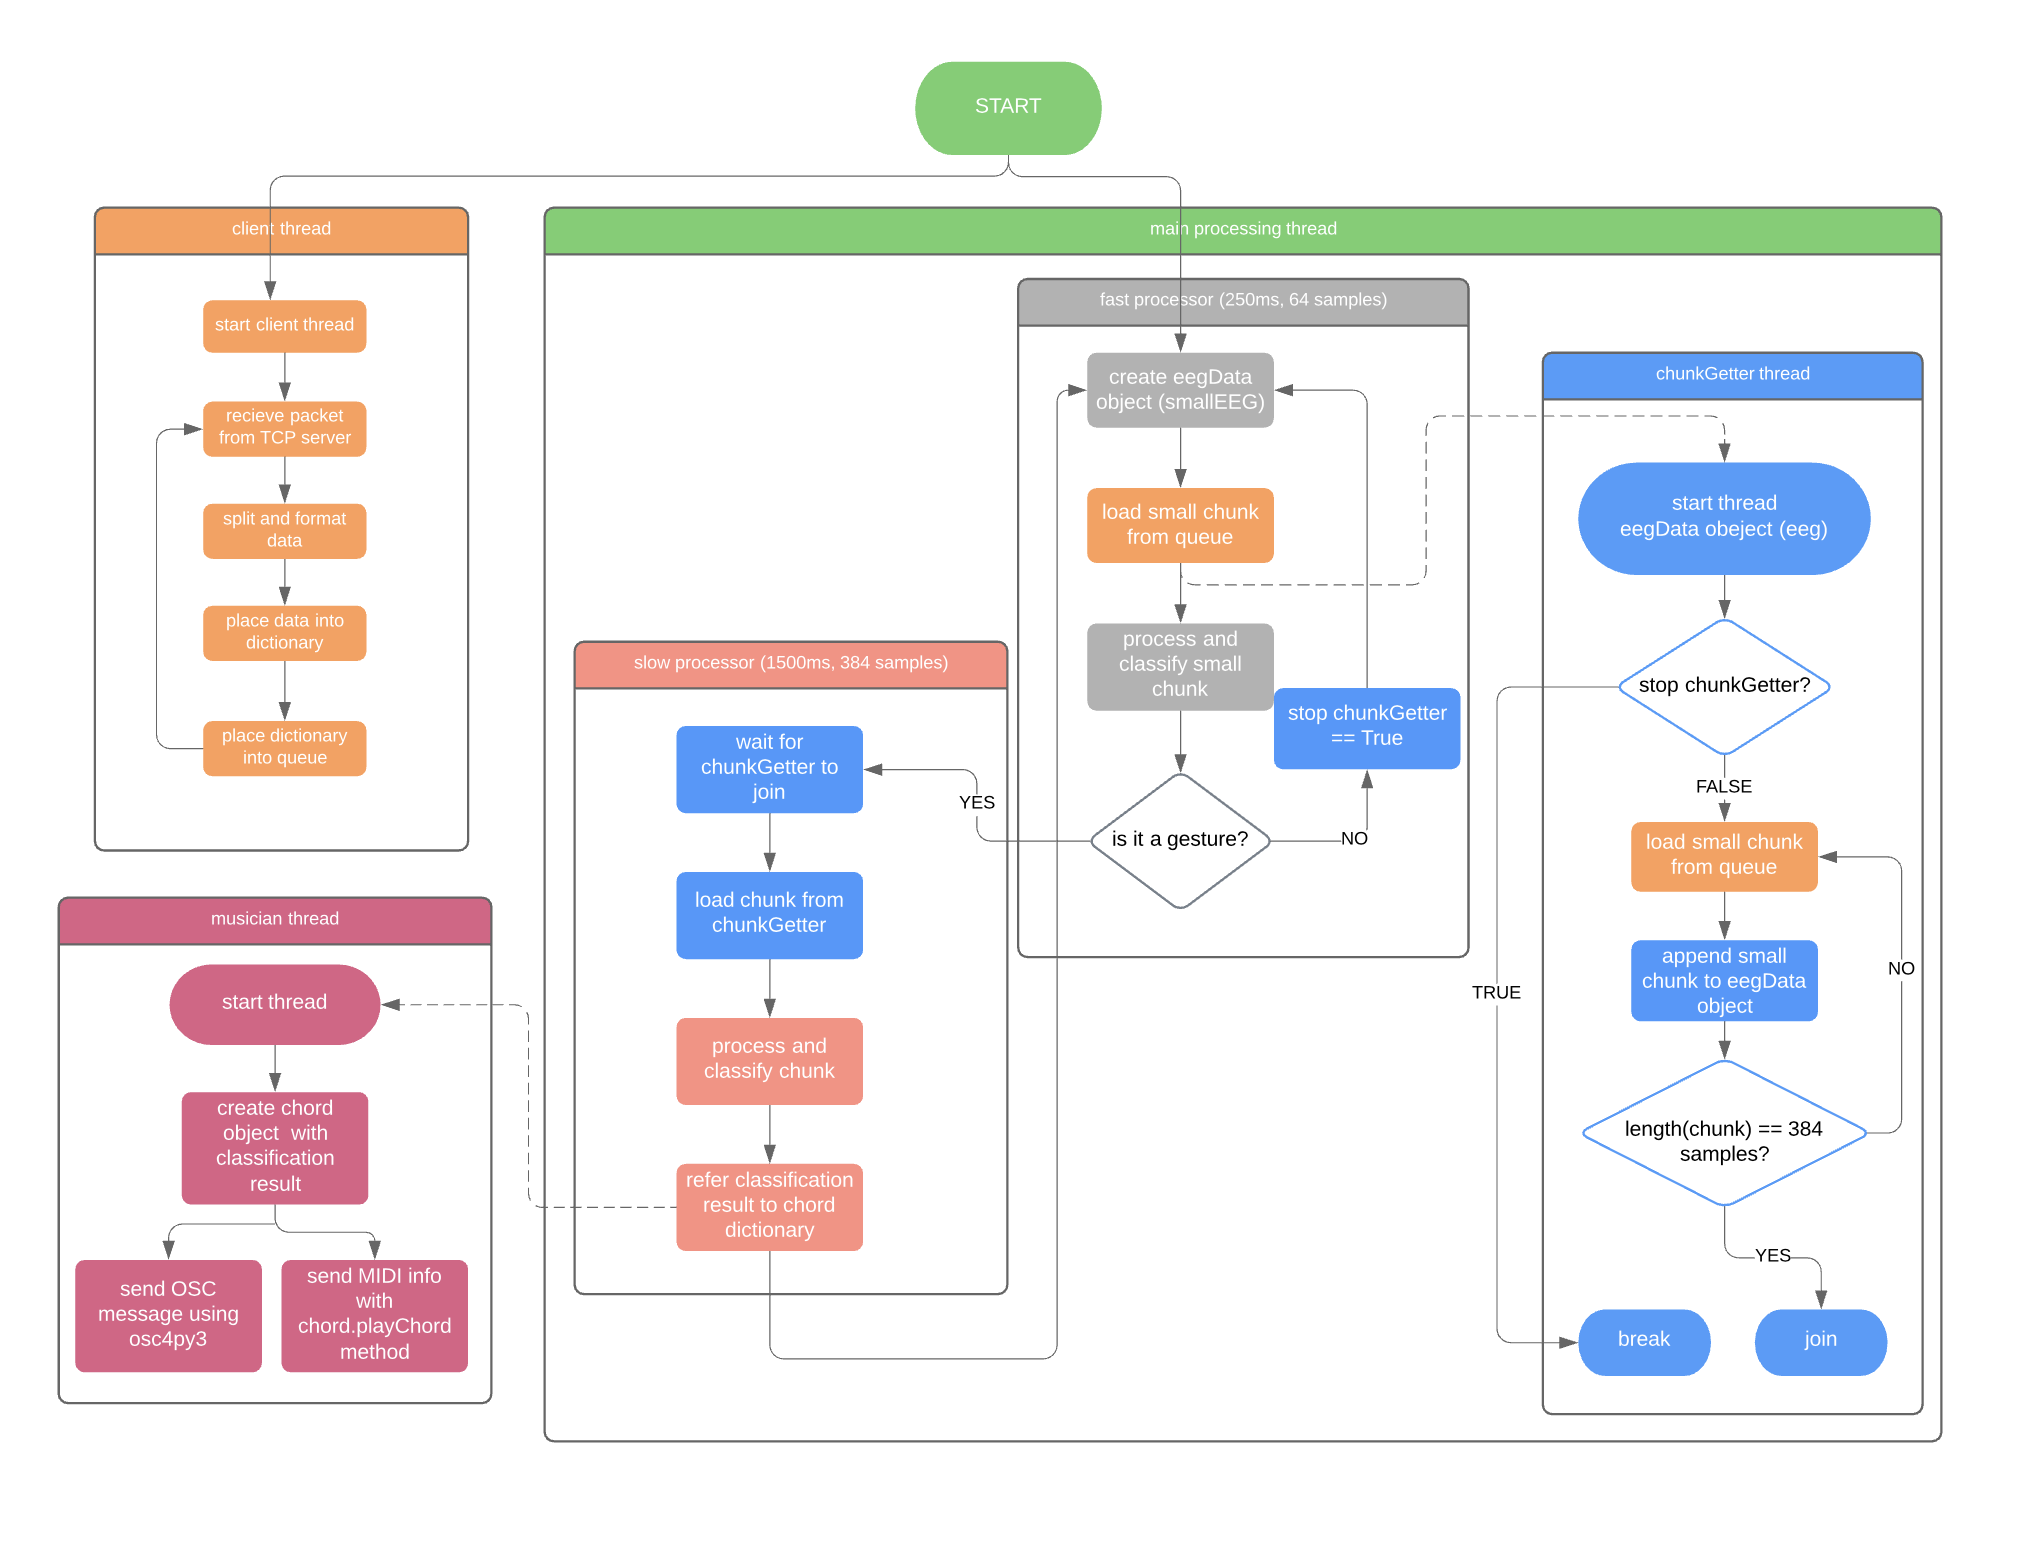
\includegraphics[width=1\columnwidth]{realTimeFlowChart.png}
	\caption{Flowchart for real-time processing with \textit{smallBrain} wake up}
	\label{fig:realTimeFlowChart}
\end{figure} 

\pagebreak

 \begin{figure}[htbp!]
	\centering
		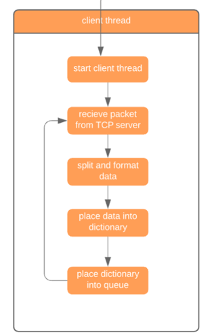
\includegraphics[width=0.25\columnwidth]{clientThread.png}
	\caption{Client Thread}
	\label{fig:clientThread}
\end{figure} 


In the client thread, a TCP client receives single EEG data packets from a live EEG stream using the EPOC+. Each packet is placed into a python queue, waiting to be retrieved by the main processing thread when requested. A copy of this queue additionally stores 128 sample buffers to be acquired by the band power processing thread. 

%In the main processing thread, a helper \textit{chunkGetter} thread takes care of receiving EEG packets from the client thread and placing them into \textit{smallChunk}s and \textit{bigChunk}s for processing by \textit{smallBrain} and \textit{bigBrain}, respectively. Once the \textit{smallChunk} array is full (250ms, 64 samples), the chunk is sent through preprocessing and feature extraction, and is classified into either a facial expression/no facial expression. While the \textit{smallChunk} array goes through preprocessing and feature extraction, the \textit{chunkGetter} thread takes care of filling up the \textit{bigChunk} array, in case the \textit{smallBrain} classifier indicates that a facial expression is present and a 320-sample chunk is needed for complete facial expression classification. 

In the main processing thread, a  \textit{chunkGetter} thread takes care of receiving EEG packets from the client thread and placing them into \textit{smallChunk}s (64 samples). A "small" ANN model (\textit{smallBrain}) classifies the \textit{smallChunk} into either a facial expression/no facial expression result. If a facial expression is found, a wake up call is sent to the \textit{bigBrain} classifier (320 samples), where facial expression classification takes place. 

The classification result is sent to a message thread, which in turn performs the predefined MIDI event indicated by the facial expression-MIDI dictionary, or sends the designated OSC message for each facial expression.

The band power processing thread takes care of retrieving 128 sample (0.5s) chunks from the client and computing band power data by using the aforementioned feature extraction algorithm. Band power values are then sent as OSC messages, where they can be used as musical control parameters in a sound processing application such as Max/MSP or SuperCollider. 

\subsection{Real Time Processing with Rising Edge Wake Up}
A flowchart for this real-time processing algorithm is provided in (Figure~\ref{fig:processorwithwakeup}). This is the algorithm implemented in the current release of the MusEEG app, as it provides a less error-prone approach to segmenting facial expressions into analyzable chunks. 

In this algorithm, the client, band power and MIDI/OSC message threads remain the same as the previous algorithm, while the main processsing thread proposes a simpler approach. 
 
 \begin{figure}[htbp]
	\centering
		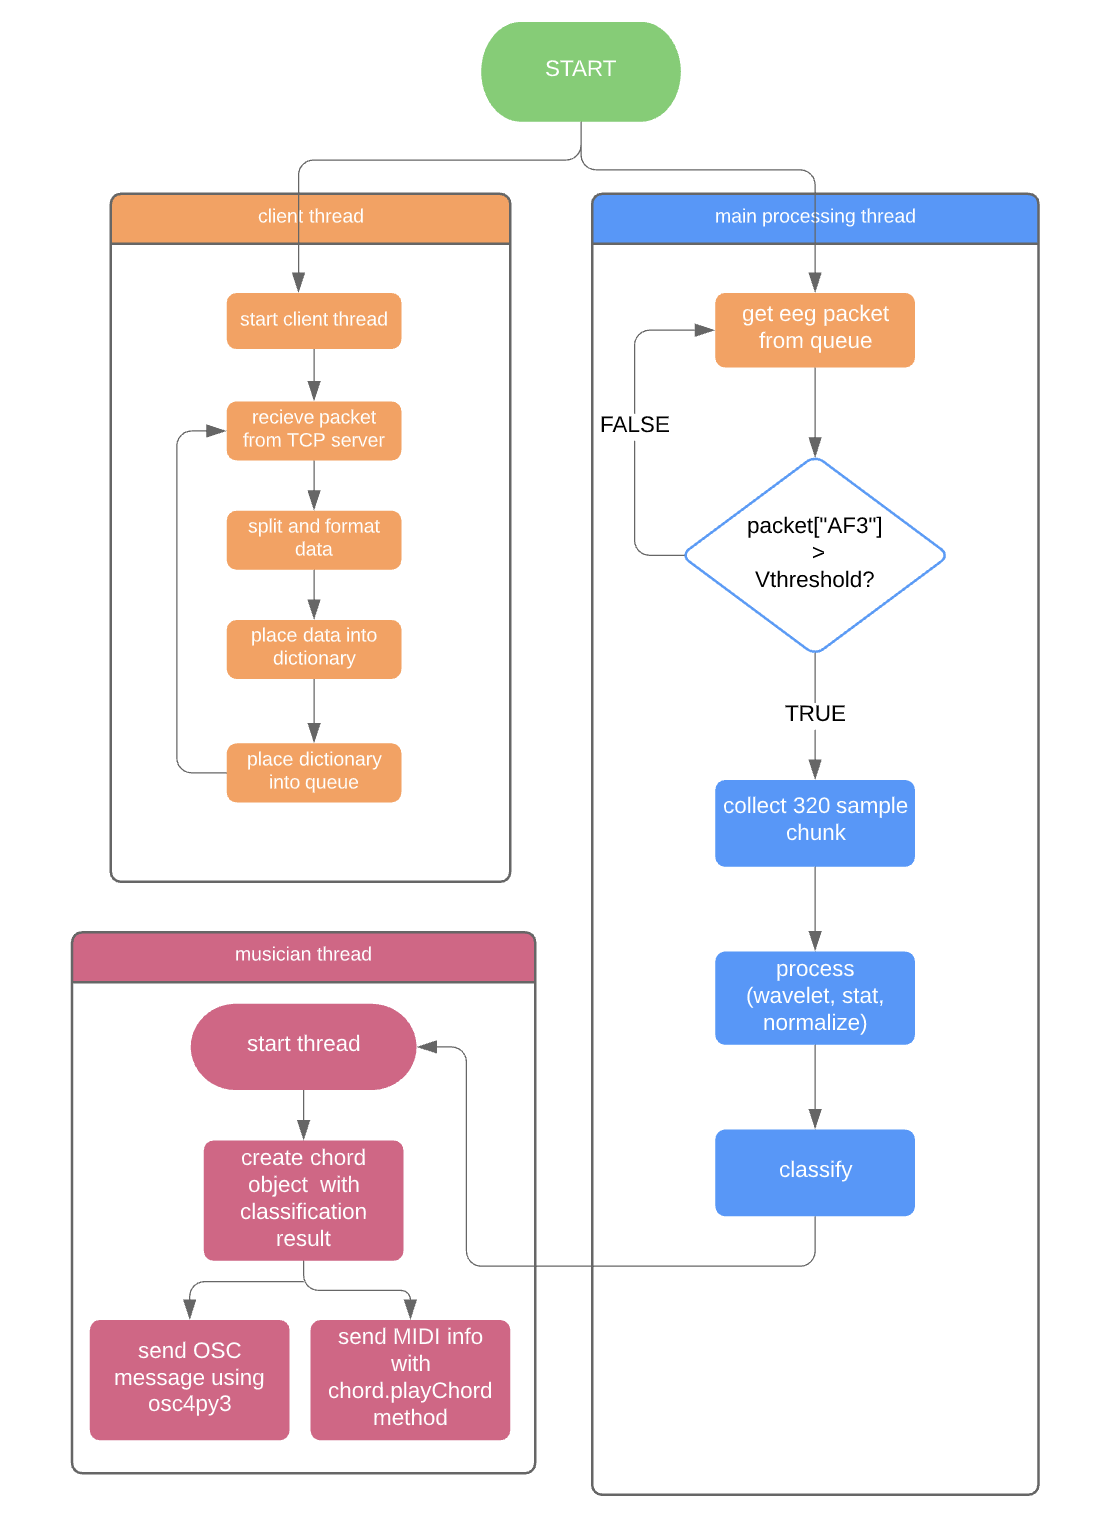
\includegraphics[width=0.75\columnwidth]{processorwithwakeup.png}
	\caption{Flowchart for real-time processing with rising edge wake up}
	\label{fig:processorwithwakeup}
\end{figure} 

In this algorithm's main processing thread, single raw EEG samples are retrieved from the client's queue and compared with a threshold voltage. If the magnitude of the packet's voltage surpasses the threshold voltage, the \textit{bigBrain} classifier is woken up, where it classifies the chunk to a facial expression. 

The classification result is sent to a message thread, which in turn performs the predefined MIDI event indicated by the facial expression-MIDI dictionary, or sends the designated OSC message for each facial expression.

Because the real time processor with \textit{smallBrain} wake up performs a full dedicated analysis on the transient data, it is able to detect facial expressions with smaller voltage magnitudes, making it a feasible option for classification of motor imagery commands. However, this can also lead to multiple false detection results that lead to a neutral classification result from the \texit{bigBrain} classifier. 

On the other hand, the real time processor with rising edge wake up is only able to detect facial expressions with high voltage magnitude, but it does so with more confidence. It was observed that the rising edge wake up algorithm provided more favorable results during unit testing. However, this algorithm might not perform well in MI classification systems. 
 
\section{Graphical User Interface}

The MusEEG Graphical User Interface (GUI) (Figure~\ref{fig:museeg-gui}) was designed to allow the user to perform the following actions: 
\begin{itemize}
\item select their desired EEG device (MusEEG currently supports the Emotiv EPOC+, and prerecorded .csv files),
\item open the MIDI menu, which contains a control center for modifying the MIDI messages assigned to facial expressions and the way the are performed on the system. 
\item load a custom \textit{bigBrain} model, and
\item view several monitoring windows for the raw EEG data, \textit{bigBrain} data chunks, and average band power over all channels. 
\end{itemize}
In addition, a post window prints classification results and other useful messages from the backend. 

\pagebreak


   \begin{figure}[htbp]
	\centering
		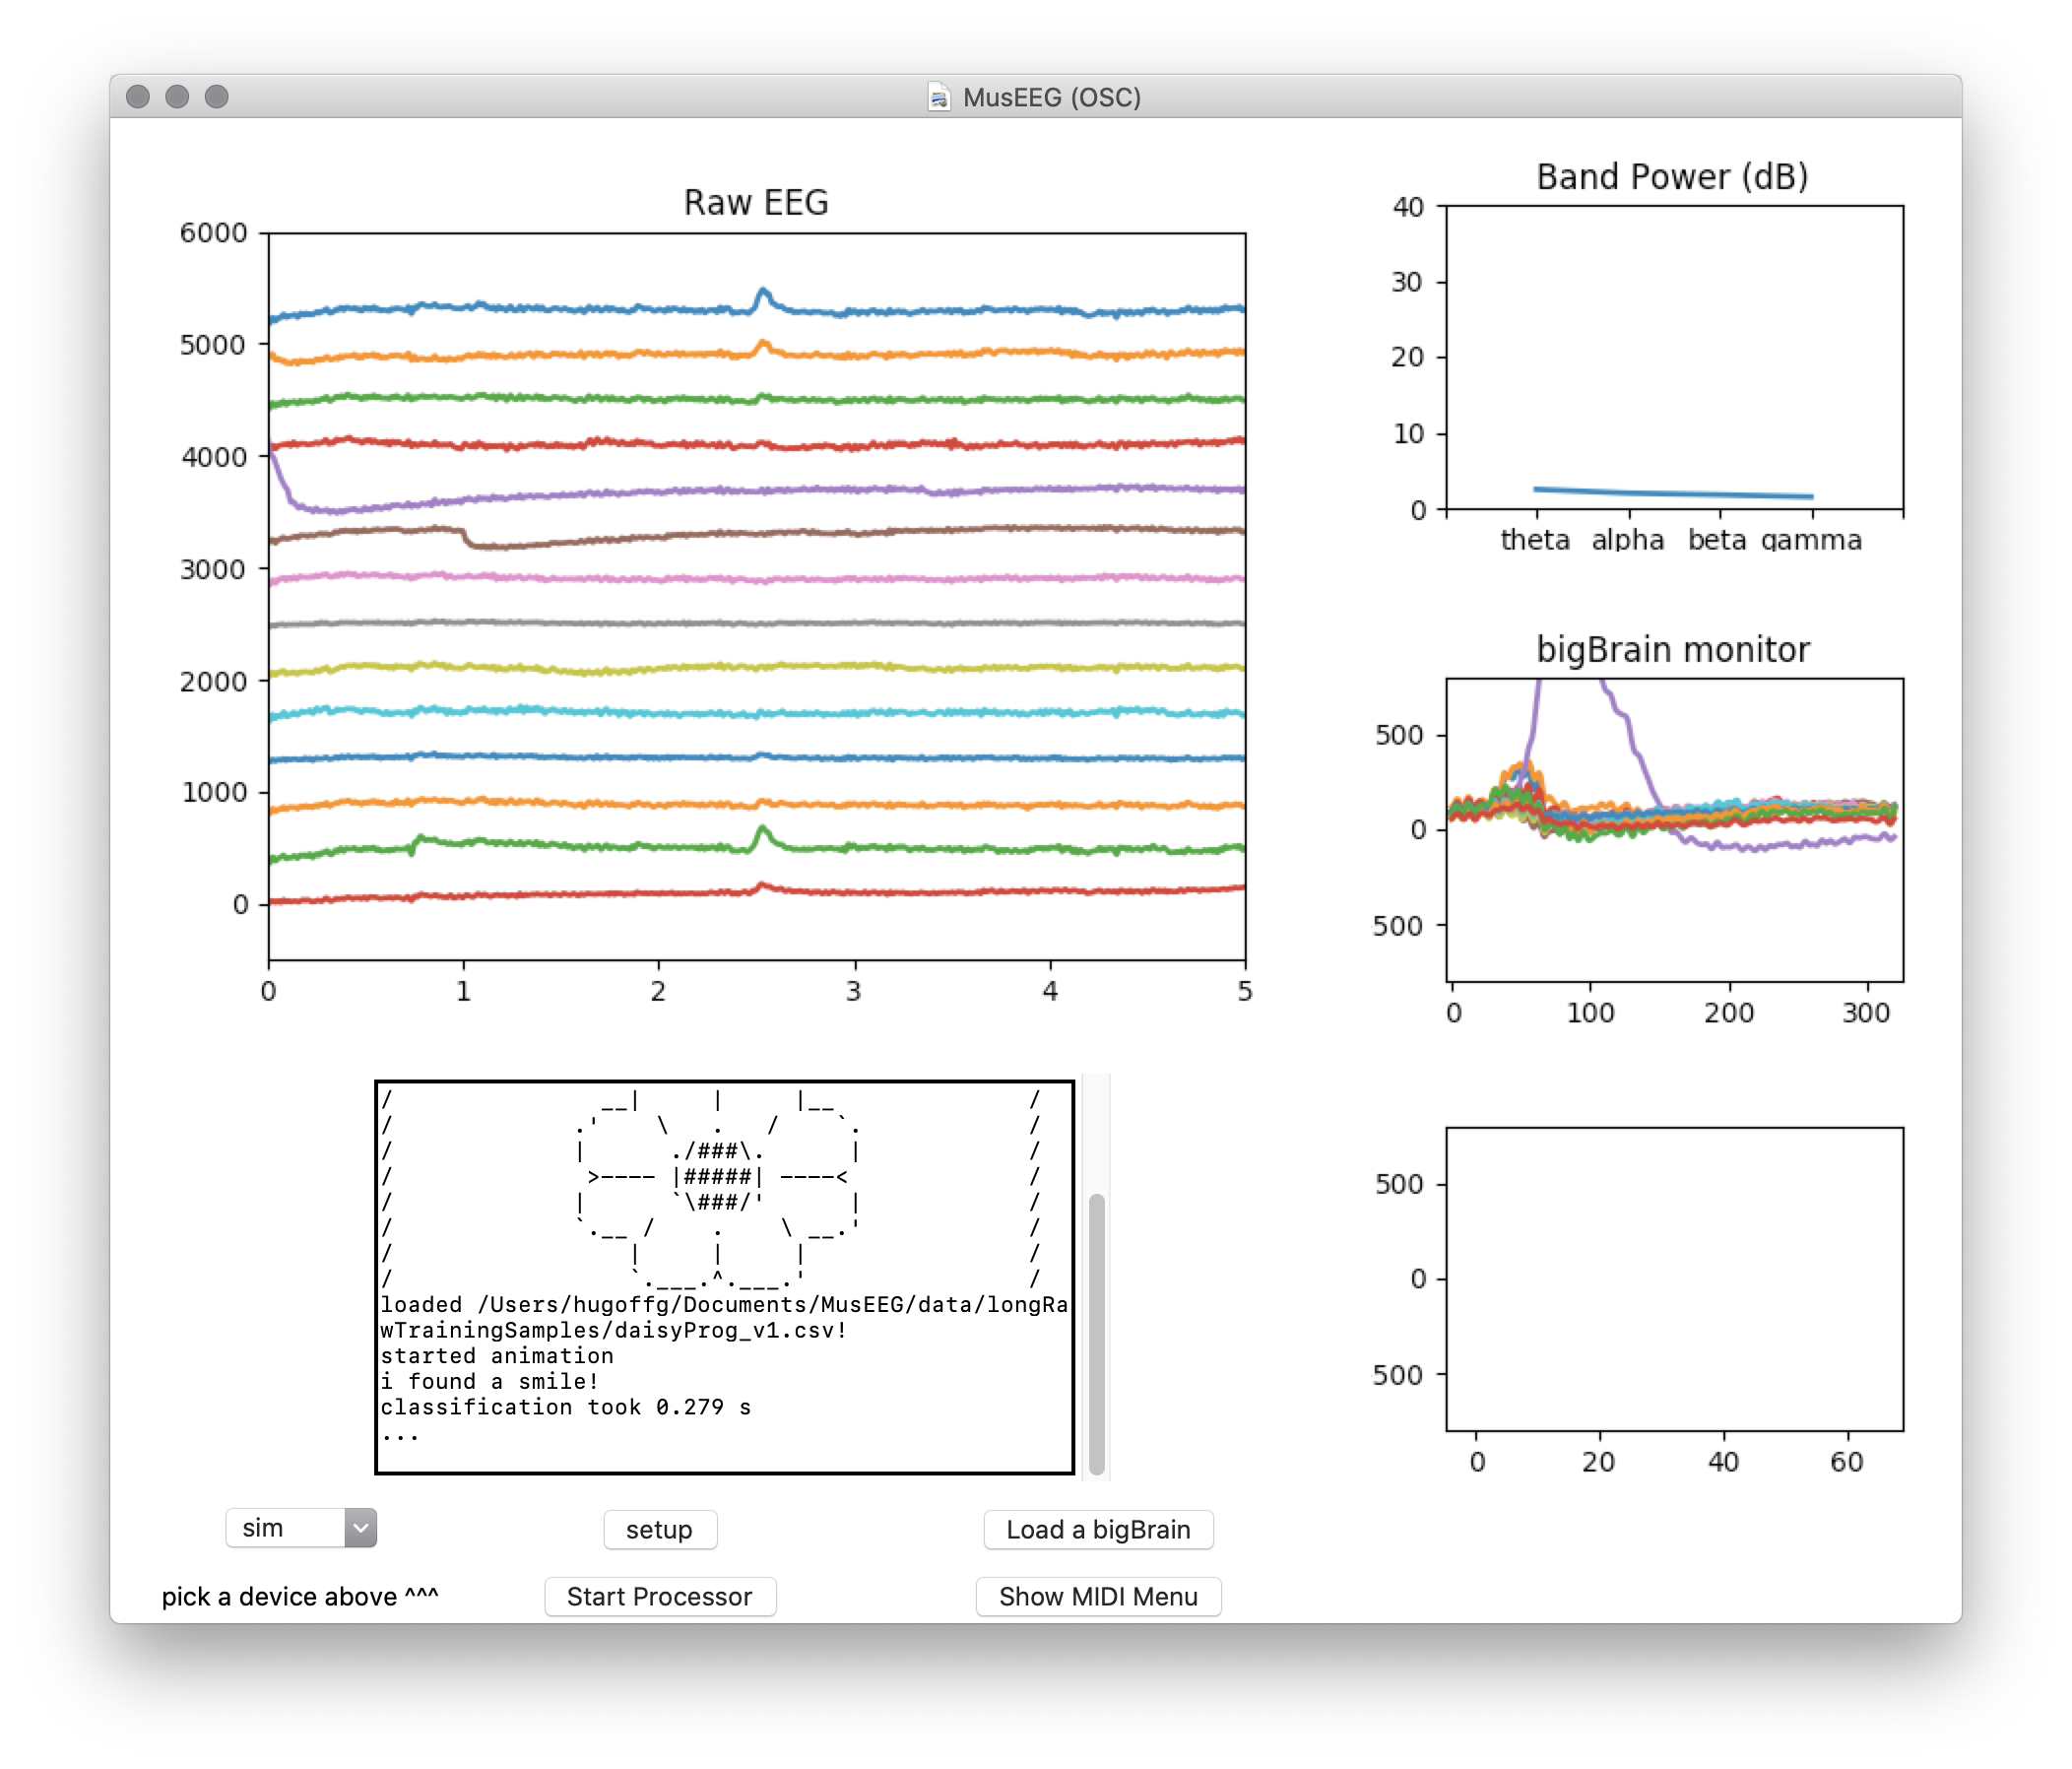
\includegraphics[width=1\columnwidth]{museeg-gui-v2.png}
	\caption{MusEEG GUI}
	\label{fig:museeg-gui}
\end{figure} 

-
\pagebreak


\subsection{The MIDI Menu}
MusEEG's MIDI menu allows users to assign custom chords to facial expressions and control the way the are performed, such as:
\begin{itemize}
\item save the current MIDI-facial expression dictionary
\item load a stored MIDI-facial expression dictionary
\item set sustain duration for non-arpeggiated chords
\item arpeggiate the chord
\item (if the chord is arppegiated) scramble the arpeggio note order
\item set the number of repeats for the arpeggio pattern. 
\end{itemize}

\begin{figure}[H]
	\centering
		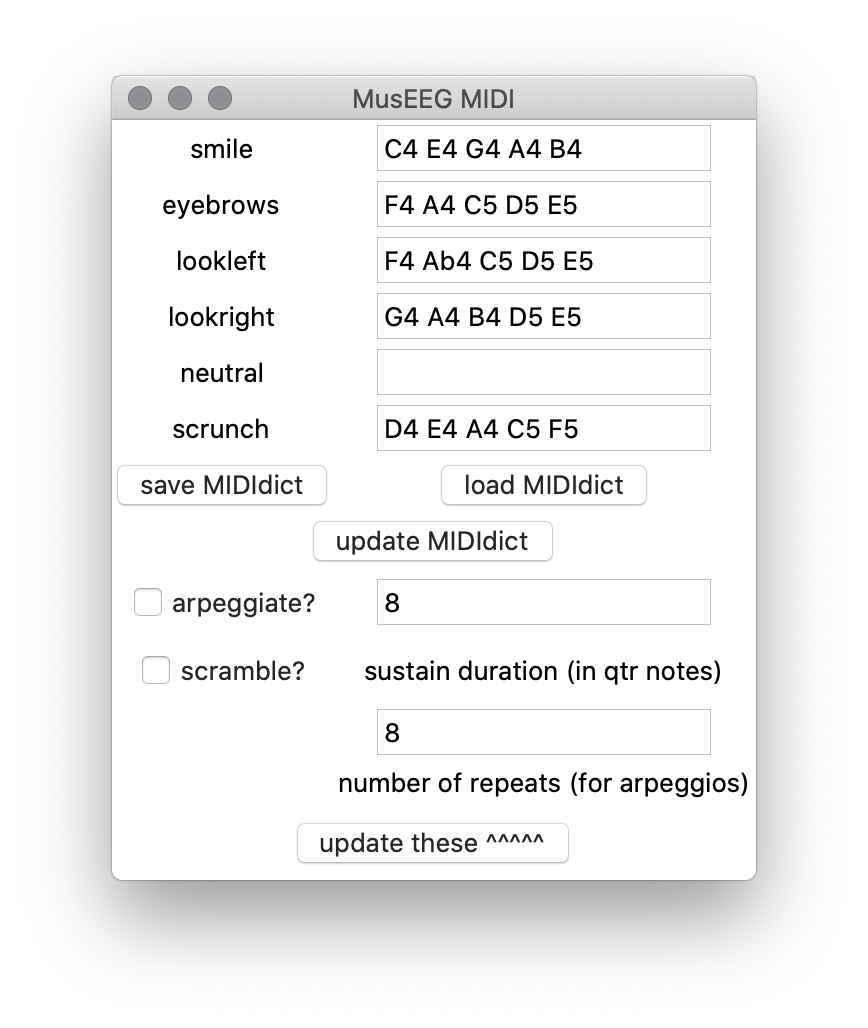
\includegraphics[width=0.6\columnwidth]{midi-menu.png}
	\caption{MIDI Menu}
	\label{fig:midi-menu}
\end{figure} 

\pagebreak

\section{Open Sound Control}
MusEEG offers a simple OSC module that wraps on top of the open-source osc4py3 library. The module introduces availability to refer user-defined OSC messages and bundles to facial expressions, and builds a client that sends said messages over a network in the message thread. 

 \begin{figure}[htbp!]
	\centering
		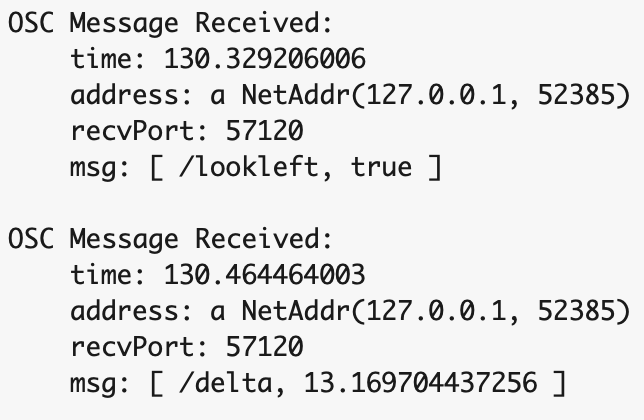
\includegraphics[width=0.7\columnwidth]{OSCmsg.png}
	\caption{MusEEG OSC message in SuperCollider}
	\label{fig:oscmsg}
\end{figure} 